\documentclass{article}
\usepackage{graphicx} 
\usepackage{fancyhdr}
\usepackage[utf8]{inputenc}
\usepackage{hyperref}
\usepackage{float}
\usepackage{pdfpages}
\usepackage{url}
\usepackage[T1]{fontenc}
\usepackage[french]{babel}
\usepackage{tabularx}
\usepackage{indentfirst}
\usepackage{mdframed}
\usepackage{amsmath}
\usepackage{pgfgantt}
\usepackage{geometry}
\usepackage{listings}
\usepackage{xcolor}

\geometry{margin=2cm}

\setlength{\headheight}{30pt}
\setlength{\headsep}{45pt}

% Style pour le code C
\definecolor{mGreen}{rgb}{0,0.6,0}
\definecolor{mGray}{rgb}{0.5,0.5,0.5}
\definecolor{mPurple}{rgb}{0.58,0,0.82}
\definecolor{background}{rgb}{0.97,0.97,0.97}

% Configuration listings pour le code C
\lstset{
    language=C,
    basicstyle=\footnotesize\ttfamily,
    keywordstyle=\color{blue},
    commentstyle=\color{green!40!black},
    stringstyle=\color{red},
    breaklines=true,
    frame=single,
    showstringspaces=false,
    numbers=left,
    numberstyle=\tiny\color{gray}
}

\begin{document}
\pagestyle{fancy}
\renewcommand{\footrulewidth}{0.2pt}
\lfoot{Alan IDMONT - Sagesse FONTAREL} 
\rfoot{Cahier de laboratoire - IE}

\begin{titlepage}
    \thispagestyle{empty}
    \begin{figure}[h]
        \begin{minipage}{0.45\textwidth}
            \begin{flushleft}
                
\includegraphics[height=2.5cm]{Logo UT.png} 
            \end{flushleft}
        \end{minipage}
        \hfill
        \begin{minipage}{0.45\textwidth}
            \begin{flushright}
                
\includegraphics[height=2.5cm]{Logo GEII.png}
            \end{flushright}
        \end{minipage}
    \end{figure}
    \newcommand{\HRule}{\rule{\linewidth}{0.5mm}}
    \center
    \textsc{\LARGE IUT de Toulouse - GEII} \\[1cm]
    \HRule \\[0.4cm]
    { \huge \bfseries Cahier de laboratoire \\ SAÉ Enregistreur numérique : \\ Partie INFO \\[0.3cm] }
    \HRule \\[0.5cm]
    Alan IDMONT - Sagesse FONTAREL
    \\[1cm]
    BUT2 GEII, Groupe ESE2, Binôme 12
    \\ [1cm]
\end{titlepage}

\newpage
\setcounter{page}{1}
\tableofcontents
\newpage

\section{Corrections principales}

Avant d'intervenir sur le code, nous avons réalisé un audit complet du projet hérité afin d'identifier les écarts par rapport au cahier des charges initial.

\subsection{Redimensionnement du buffer d'échantillonnage}

Le code existant utilisait un tableau limité à 20~000 échantillons, alors que la RAM du STM32L476 permettait d'atteindre la capacité demandée de 95~ko. Nous avons donc recalculé la taille optimale du buffer.

\textbf{Correction apportée :} Le tableau a été redimensionné à 45~000 échantillons de type \texttt{uint16\_t}, ce qui représente environ 90~ko de mémoire utilisée.

\begin{lstlisting}[caption=Modification de la taille du buffer (main.c)]
static uint16_t tabEchantillons[45000]; // Redimensionnement pour utiliser la RAM disponible
donnees_t mesDonnees = {ARRET, false, tabEchantillons, 45000, 0, -1, DIRECT};
\end{lstlisting}

\subsection{Restructuration de la boucle principale}

La boucle principale \texttt{while(1)} présentait un fonctionnement bloquant inadapté à une application temps réel. Nous l'avons restructurée pour qu'elle s'exécute de manière non-bloquante, synchronisée sur le Timer 7.

Pour évaluer la charge processeur, nous avons ajouté un basculement de GPIO (\texttt{VisuPin1}) permettant d'observer à l'oscilloscope le temps d'exécution réel par rapport à la période d'échantillonnage $T_{ech}$.

\begin{lstlisting}[caption=Boucle principale cadencée par le Timer 7]
while (1) {
    if (__HAL_TIM_GET_FLAG(&htim7, TIM_FLAG_UPDATE)) {
        menu(&maConfig, &mesDonnees);
        // Gestion du bouton bleu pour acquitter l'action
        if (HAL_GPIO_ReadPin(btn_Bleu_GPIO_Port, btn_Bleu_Pin) == GPIO_PIN_RESET)
            mesDonnees.etatBouton = true;

        HAL_GPIO_WritePin(VisuPin1_GPIO_Port, VisuPin1_Pin, GPIO_PIN_SET);
        switch (mesDonnees.mode) {
            case RECOPIE: modeRecopie(&maConfig, &mesDonnees); break;
            case ACQUISITION: modeAcquisition(&maConfig, &mesDonnees); break;
            case RESTITUTION: modeRestitution(&maConfig, &mesDonnees); break;
            default: break;
        }
        HAL_GPIO_WritePin(VisuPin1_GPIO_Port, VisuPin1_Pin, GPIO_PIN_RESET);
        __HAL_TIM_CLEAR_FLAG(&htim7, TIM_FLAG_UPDATE);
    }
}
\end{lstlisting}

\section{Mode Recopie : Validation expérimentale}

Le mode recopie doit transférer en temps réel les valeurs de l'ADC vers le DAC, sans stockage intermédiaire. L'implémentation initiale utilisait un mécanisme bloquant qui ne respectait pas les contraintes temporelles.

\textbf{Solution retenue :} Nous avons utilisé la fonction \texttt{HAL\_ADC\_PollForConversion} avec un timeout réduit à 1~ms afin de garantir que le traitement reste dans la fenêtre d'échantillonnage $T_{ech}$.

\begin{figure}[H]
    \centering
    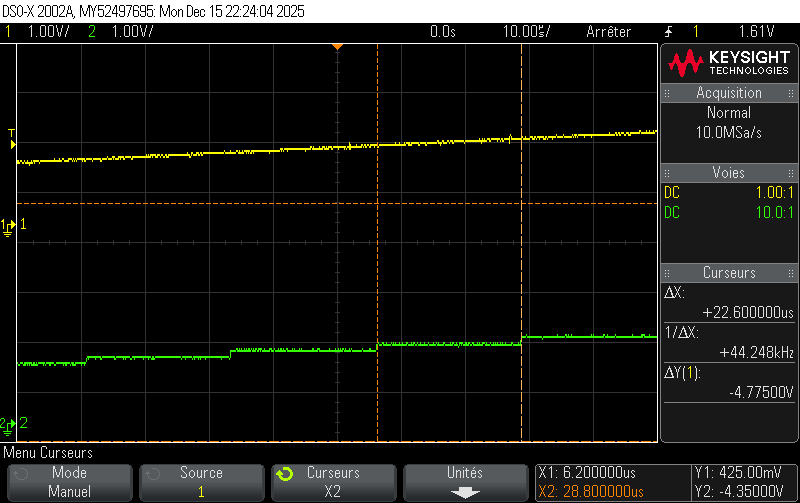
\includegraphics[width=0.75\textwidth]{Recopie_simple_44.1k_correct_2.png}
    \caption{Vérification de la fréquence d'échantillonnage à l'oscilloscope}
\end{figure}

Les relevés oscilloscopiques confirment la précision du système : pour une fréquence d'échantillonnage de 44,1~kHz, nous mesurons une période de 22,6~$\mu$s, correspondant à environ 44,248~kHz. L'écart reste bien inférieur à la marge de 0,1~\% spécifiée. Le signal vert illustre les paliers caractéristiques de la reconstruction par le DAC.

\section{Mode Acquisition : Diagnostic et résolution}

\subsection{Identification du problème}

L'analyse du code d'acquisition a révélé un problème de persistance de l'index d'écriture. À chaque appel par le timer, la fonction redémarrait avec un index remis à zéro, ce qui empêchait tout stockage cohérent des échantillons.

\subsection{Validation par le débogueur}

Le mode Debug de STM32CubeIDE nous a permis d'observer en temps réel l'évolution des variables locales et du contenu de la RAM. Les captures suivantes illustrent le processus d'acquisition.

\begin{figure}[H]
    \centering
    \begin{minipage}{0.32\textwidth}
        \centering
        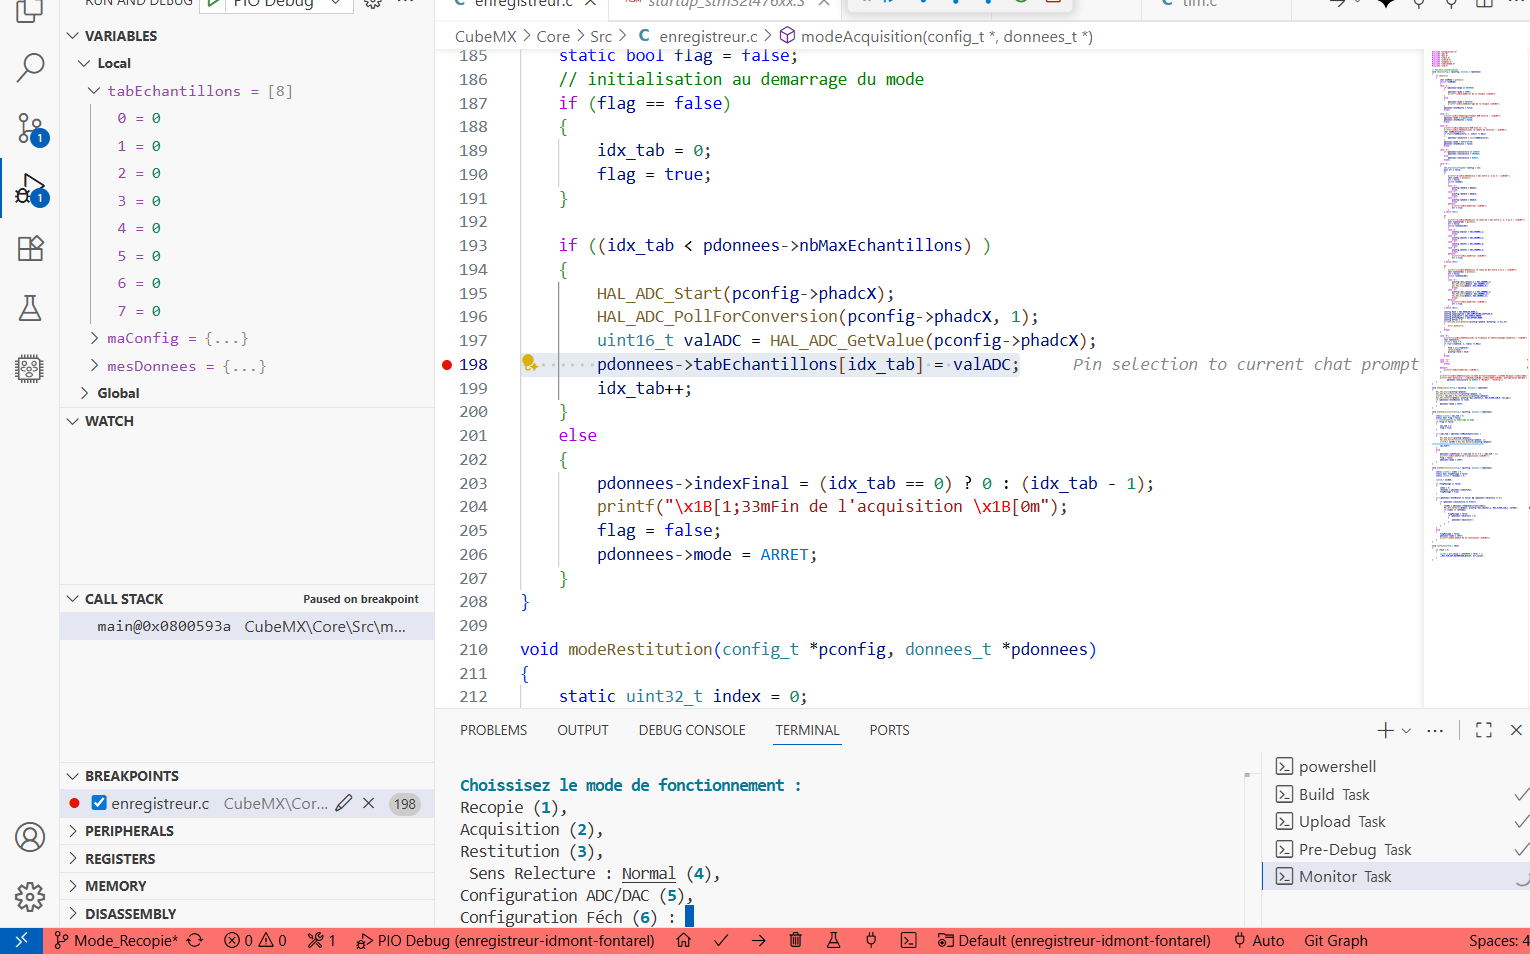
\includegraphics[width=\textwidth]{Avant acquisition.png}
        \caption{État initial}
    \end{minipage}
    \begin{minipage}{0.32\textwidth}
        \centering
        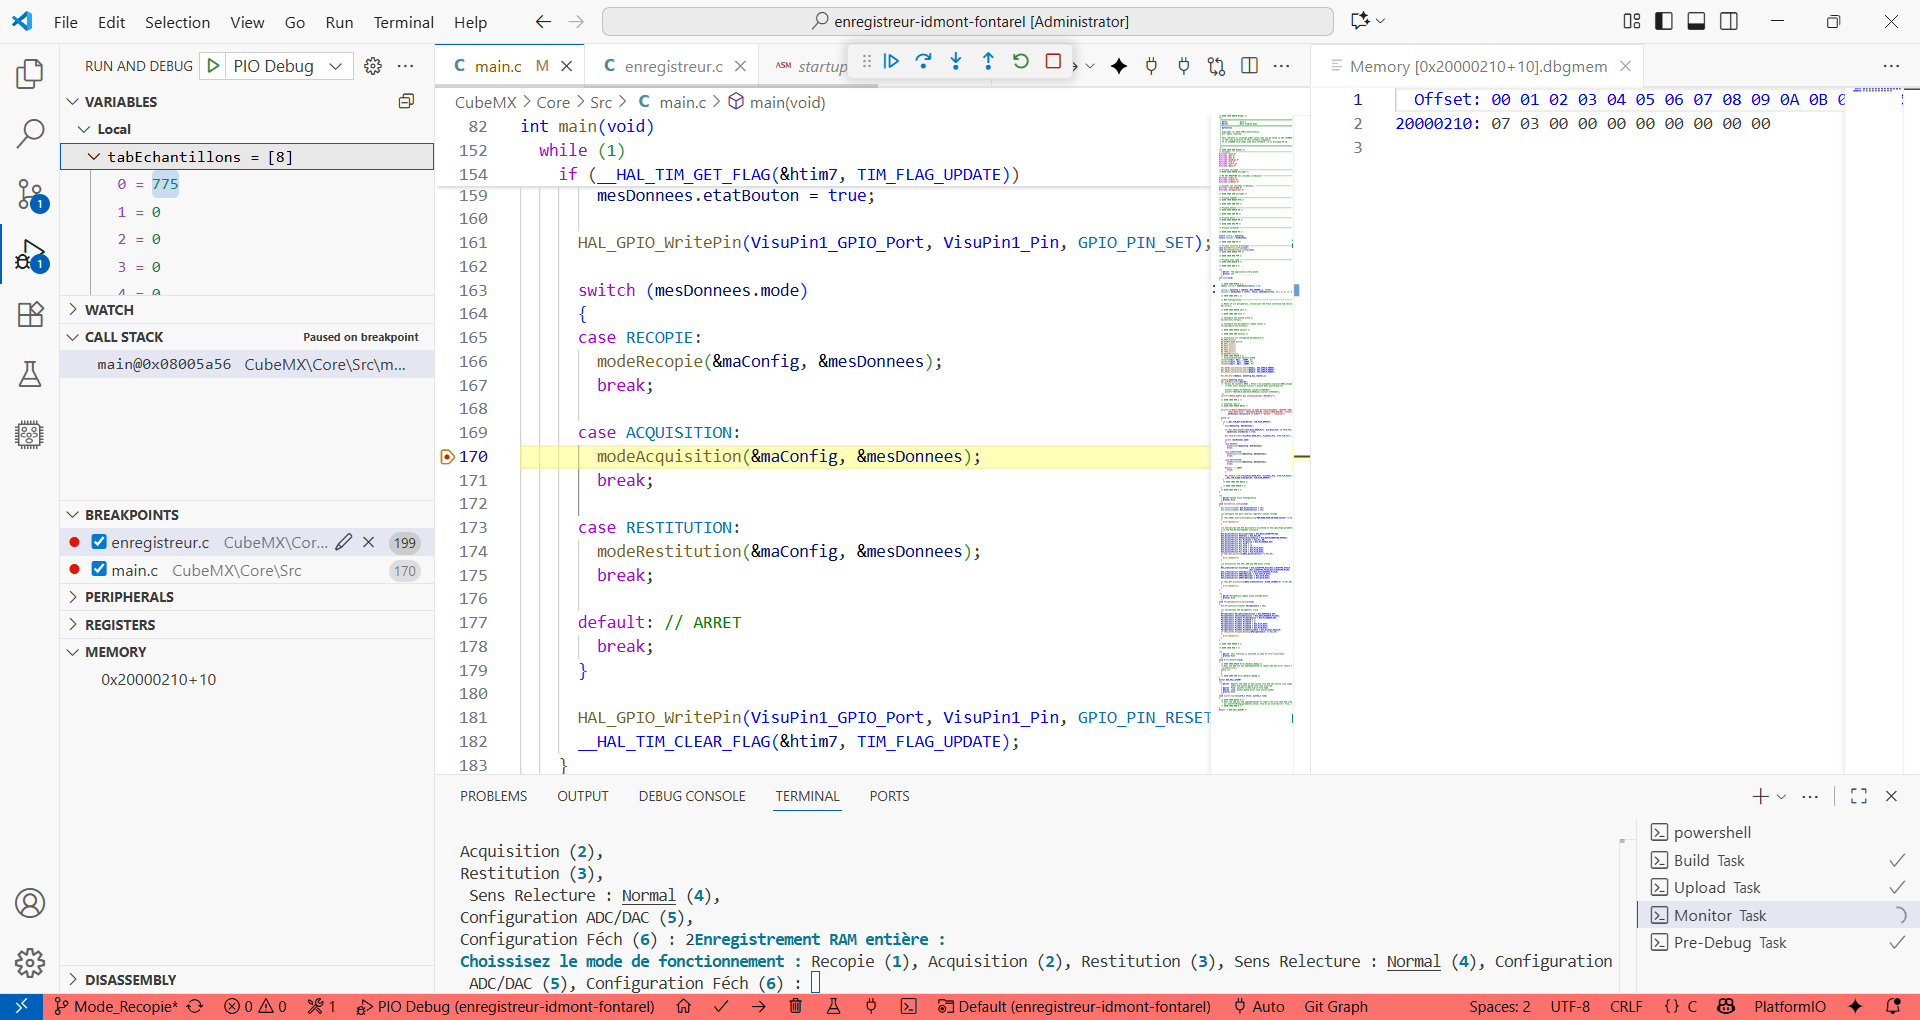
\includegraphics[width=\textwidth]{Après 1 acquisition.png}
        \caption{Premier échantillon (775)}
    \end{minipage}
    \begin{minipage}{0.32\textwidth}
        \centering
        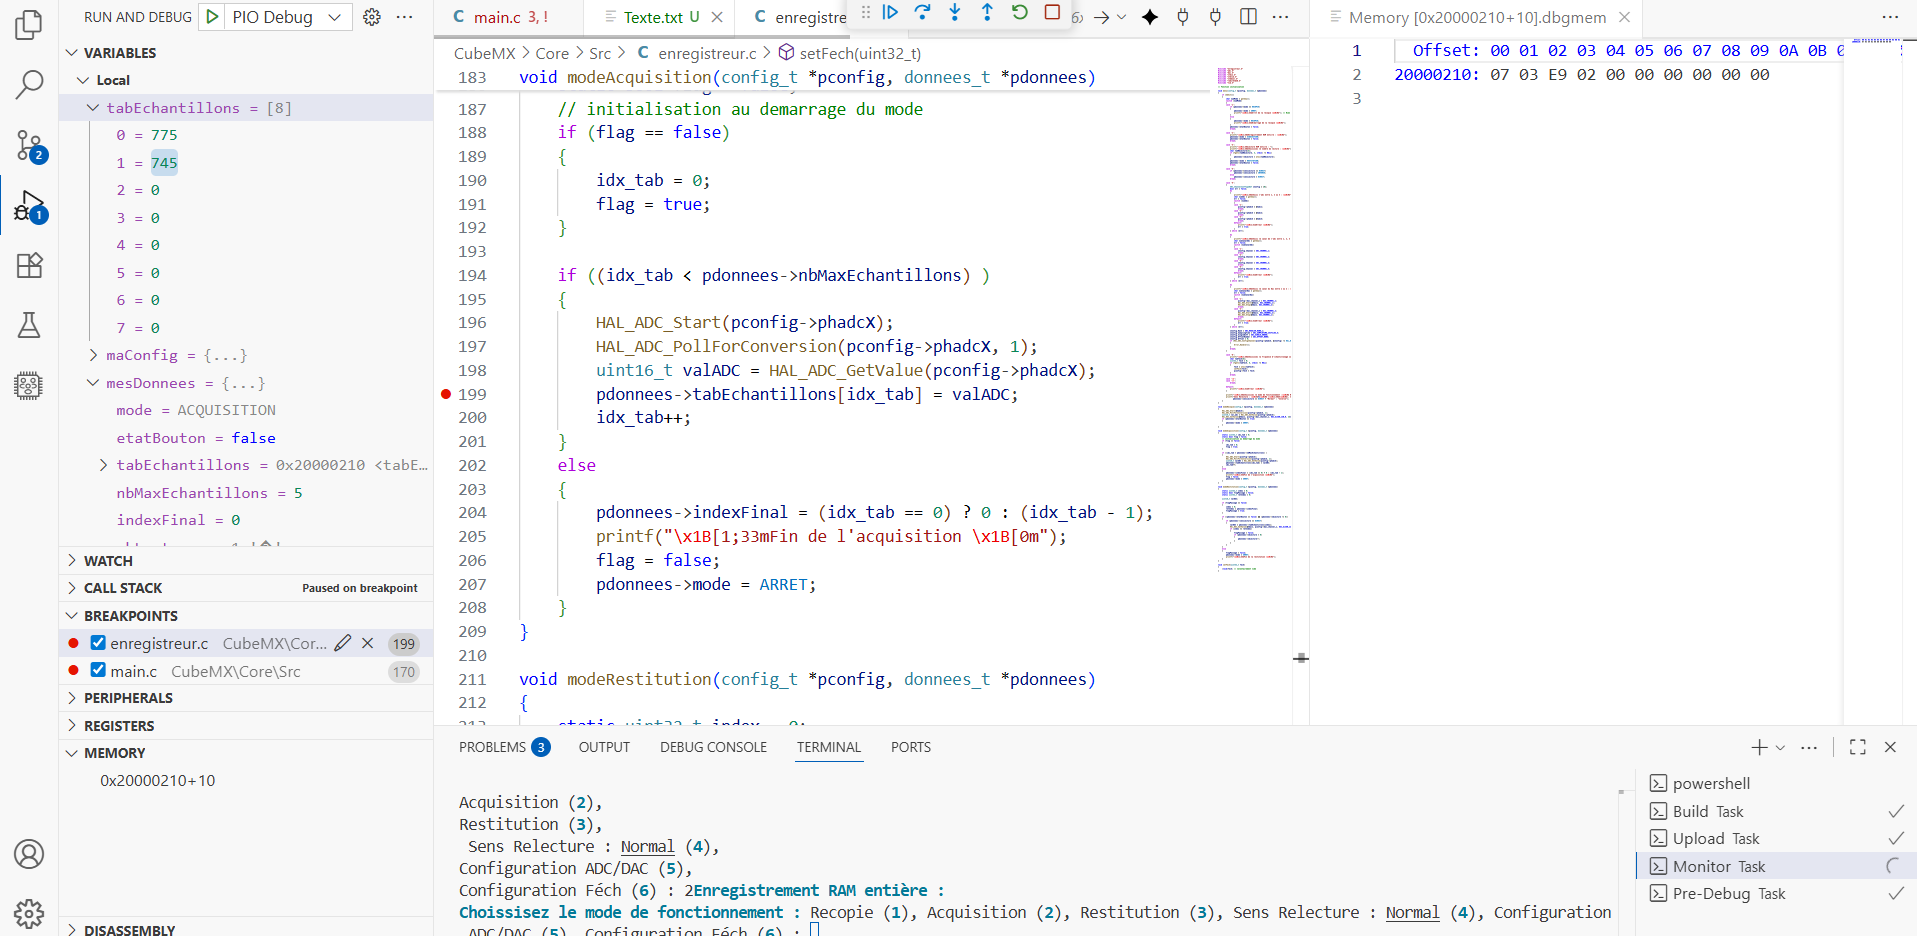
\includegraphics[width=\textwidth]{Après 2 acquisitions.png}
        \caption{Deuxième échantillon (745)}
    \end{minipage}
\end{figure}

La vue \texttt{Variables} confirme l'incrémentation correcte de \texttt{idx\_tab} (0 $\rightarrow$ 1 $\rightarrow$ 2) et la vue \texttt{Memory} montre le stockage effectif des valeurs (0x0307 correspond à 775 en décimal).

\subsection{Correction mise en œuvre}

Nous avons déclaré l'index en tant que variable statique, avec un mécanisme de réinitialisation contrôlé par un flag lors du passage au mode ACQUISITION.

\begin{lstlisting}[caption=Fonction d'acquisition corrigée]
static uint32_t idx_tab = 0;
static bool flag = false;

if (flag == false) { // Reinitialisation en debut de mode uniquement
    idx_tab = 0;
    flag = true;
}

if ((idx_tab < pdonnees->nbMaxEchantillons) && (pdonnees->etatBouton == false)) {
    pdonnees->tabEchantillons[idx_tab] = valADC;
    idx_tab++;
} else { 
    pdonnees->indexFinal = idx_tab;
    flag = false;
    pdonnees->mode = ARRET;
}
\end{lstlisting}

\section{Mode Restitution : Résolution du blocage}

\subsection{Analyse du dysfonctionnement}

Les tests ont montré que la restitution ne produisait aucun signal en sortie. L'analyse avec le débogueur a révélé que \texttt{indexFinal} restait à zéro, empêchant ainsi toute lecture du buffer.

\begin{figure}[H]
    \centering
    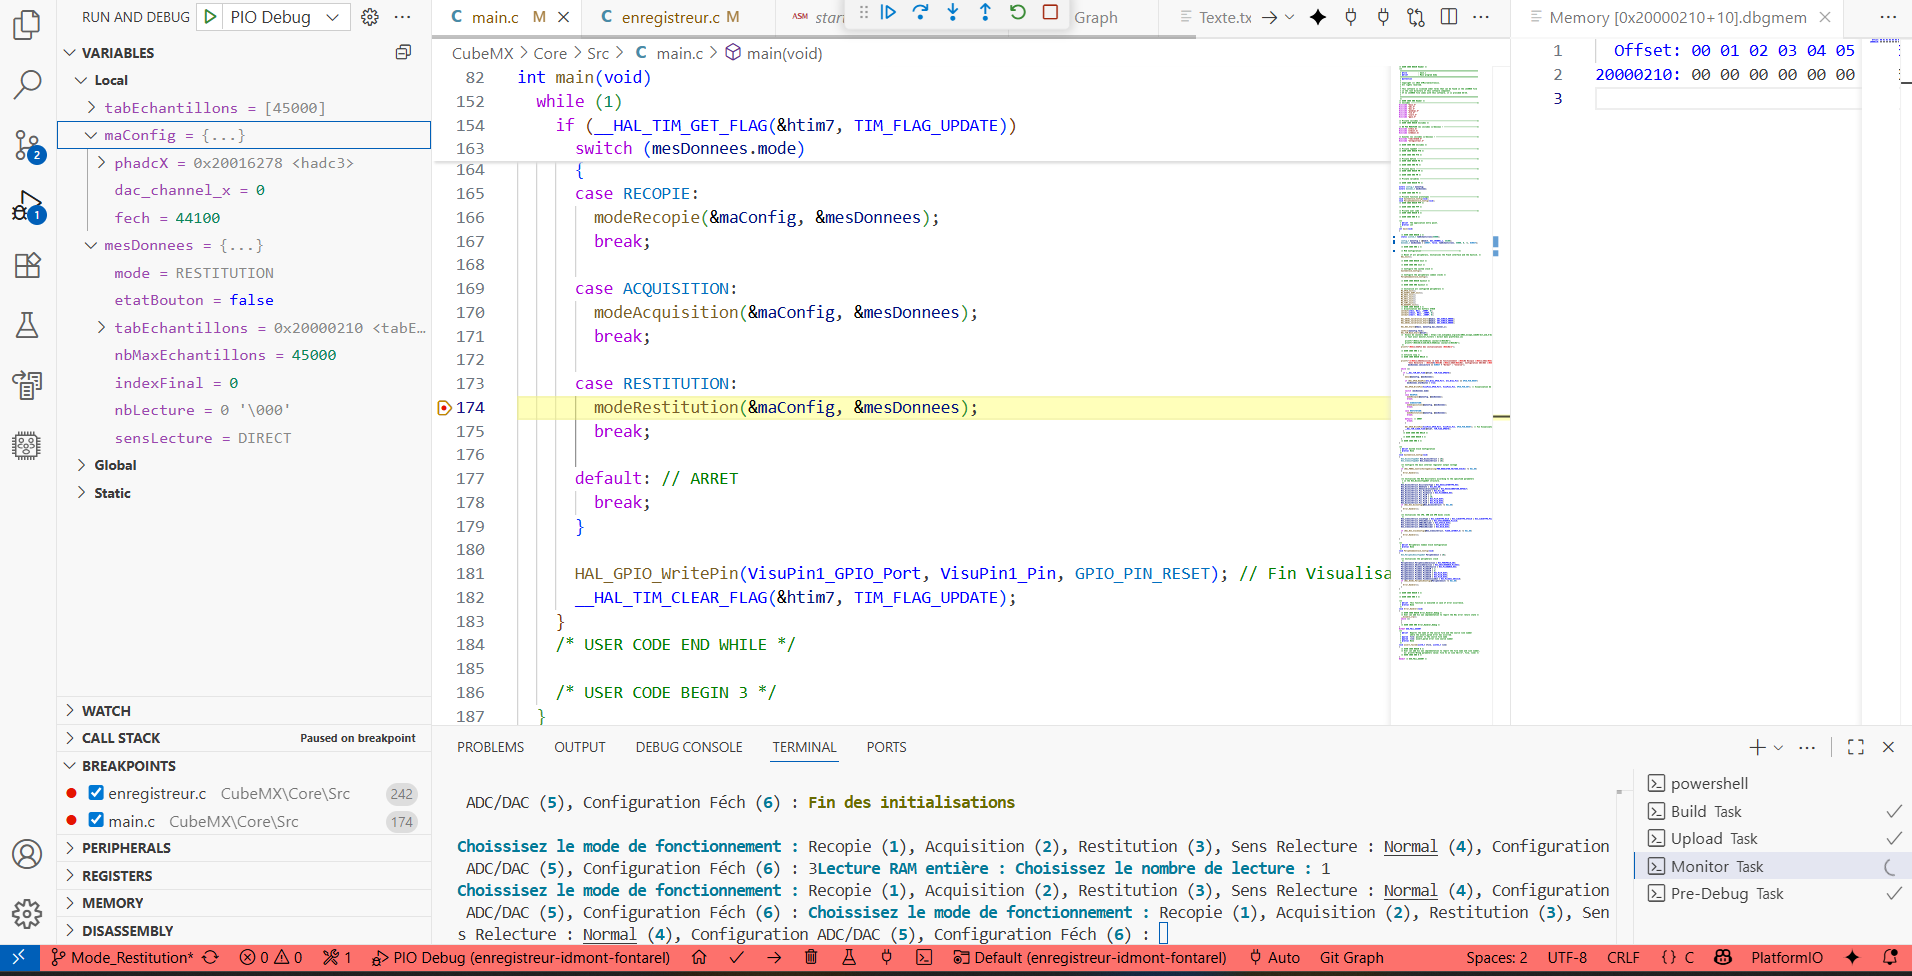
\includegraphics[width=0.7\textwidth]{Restitution_Index_bloqué.png}
    \caption{État des variables : indexFinal = 0 bloque la restitution}
\end{figure}

\subsection{Implémentation de la solution}

Nous avons ajouté une vérification de \texttt{indexFinal} en entrée de fonction, avec retour automatique au mode ARRET si cette valeur est nulle. De plus, nous gérons maintenant le nombre de lectures (\texttt{nbLecture}) pour permettre la répétition du signal enregistré.

\begin{lstlisting}[caption=Fonction de restitution ]
static uint32_t index = 0;
static bool flagPassage = false;

if (flagPassage == false) {
    if (pdonnees->indexFinal == 0) { 
        pdonnees->mode = ARRET; 
        return; 
    }
    index = 0;
    flagPassage = true;
}

if (pdonnees->etatBouton == false && pdonnees->nbLecture != 0) {
    HAL_DAC_SetValue(&hdac1, pconfig->dac_channel_x, DAC_ALIGN_12B_R, 
                     pdonnees->tabEchantillons[index]);
    index++;
    
    if (index >= pdonnees->indexFinal) { 
        if (pdonnees->nbLecture > 0) pdonnees->nbLecture--;
        index = 0;
        if (pdonnees->nbLecture == 0) { 
            flagPassage = false; 
            pdonnees->mode = ARRET; 
        }
    }
}
\end{lstlisting}

\section{Conception : Architecture Foreground / Background}

L'objectif de cette phase était de migrer d'une architecture par scrutation (\textit{polling}) vers une architecture "Temps Réel" véritable. La boucle principale est désormais libérée pour l'interface utilisateur, tandis que le traitement critique est déporté dans le contexte des interruptions.

\subsection{Gestion des Drapeaux matériels (Flags) et NVIC}
Comme souligné par le professeur, la gestion des drapeaux (\textit{flags}) a été un point d'apprentissage majeur. 
\begin{itemize}
    \item \textbf{Analyse :} Dans notre ancienne version, nous utilisions \texttt{\_\_HAL\_TIM\_GET\_FLAG} dans le \texttt{while(1)}. 
    \item \textbf{Modification :} Avec les interruptions, le flag \texttt{UIF} (Update Interrupt Flag) est géré automatiquement par le matériel et la couche HAL dans le fichier \texttt{stm32l4xx\_it.c}. L'appel à \texttt{HAL\_TIM\_IRQHandler(\&htim7)} acquitte le drapeau et lance notre \texttt{Callback}.
\end{itemize}

\section{Structure de Données et Initialisation Globale}

Pour permettre la communication entre le menu (Background) et le traitement audio (Foreground), les variables ont été repositionnées en globales avec l'usage impératif du mot-clé \texttt{volatile}.

\subsection{Définitions dans enregistreur.h}
Nous avons modifié le type \texttt{donnees\_t} pour intégrer la machine à états des zones et le sens de lecture.

\begin{lstlisting}[caption={Extrait de enregistreur.h}]
#define FREQ_CLOCK 80000000
#define TAILLE_RAM_L476 95000 // Limite physique de la puce

typedef enum { ZONE_A, ZONE_B } zone_t;
enum ModeFct { ARRET, RECOPIE, ACQUISITION, RESTITUTION };
enum SensRestitution { DIRECT, INVERSE };

typedef struct {
    enum ModeFct mode;
    bool etatBouton;
    uint16_t *tabEchantillonsA; // Pointeur Zone A
    uint16_t *tabEchantillonsB; // Pointeur Zone B
    uint32_t nbMaxEchantillons;
    zone_t zoneActive;          // Machine a etats ZONE
    uint32_t indexFinalA;       
    uint32_t indexFinalB;       
    int8_t nbLecture;           
    enum SensRestitution sensLecture; 
} donnees_t;
\end{lstlisting}

\subsection{Implémentation dans main.c}
L'usage de \texttt{extern} permet d'accéder aux handles matériels depuis la couche applicative.

\begin{lstlisting}[caption={Initialisation globale dans main.c}]
/* USER CODE BEGIN 0 */
static uint16_t tabEchantillonsA[20000];
static uint16_t tabEchantillonsB[20000];

// volatile pour garantir la lecture memoire malgré les IT
volatile config_t maConfig = {&hadc3, DAC_CHANNEL_1, 1000};
volatile donnees_t mesDonnees = {ARRET, false, tabEchantillonsA, tabEchantillonsB, 15000, ZONE_A, 0, 0, -1, DIRECT};
/* USER CODE END 0 */
\end{lstlisting}

\section{Fonction 1 : Architecture par Interruptions (Timer 7)}

\textbf{La logique :} Passer d'un mode bloquant à une architecture "Temps Réel". Le signal audio est désormais cadencé par le Timer 7. À chaque "tick", le processeur suspend le menu console pour traiter l'échantillon. C'est la garantie d'une fréquence d'échantillonnage ($F_{ech}$) parfaitement stable.

\textbf{Mise en œuvre du code :}
La routine $HAL_TIM_PeriodElapsedCallback$ devient le centre névralgique. Elle gère la machine à états $$(RECOPIE, ACQUISITION, RESTITUTION)$$ sans modifier la signature des fonctions existantes.

\begin{lstlisting}[caption={Callback de traitement audio dans enregistreur.c}]
void HAL_TIM_PeriodElapsedCallback(TIM_HandleTypeDef *htim) {
    if (htim->Instance == TIM7) {
        // SET Pin pour mesurer precisement la charge CPU sur VisuPin1
        HAL_GPIO_WritePin(VisuPin1_GPIO_Port, VisuPin1_Pin, GPIO_PIN_SET); 

        switch (mesDonnees.mode) {
            case RECOPIE: 
                modeRecopie(&maConfig, &mesDonnees); 
                break;
            case ACQUISITION: 
                modeAcquisition(&maConfig, &mesDonnees); 
                break;
            case RESTITUTION: 
                modeRestitution(&maConfig, &mesDonnees); 
                break;
            default: break;
        }
        // RESET Pin pour quantifier le temps d'execution reel
        HAL_GPIO_WritePin(VisuPin1_GPIO_Port, VisuPin1_Pin, GPIO_PIN_RESET); 
    }
}
\end{lstlisting}

\textbf{Tests et Résultats :}
L'utilisation de \texttt{SET/RESET} au lieu d'un \texttt{Toggle} permet de voir la "charge CPU" à l'oscilloscope.
\begin{figure}[H]
    \centering
    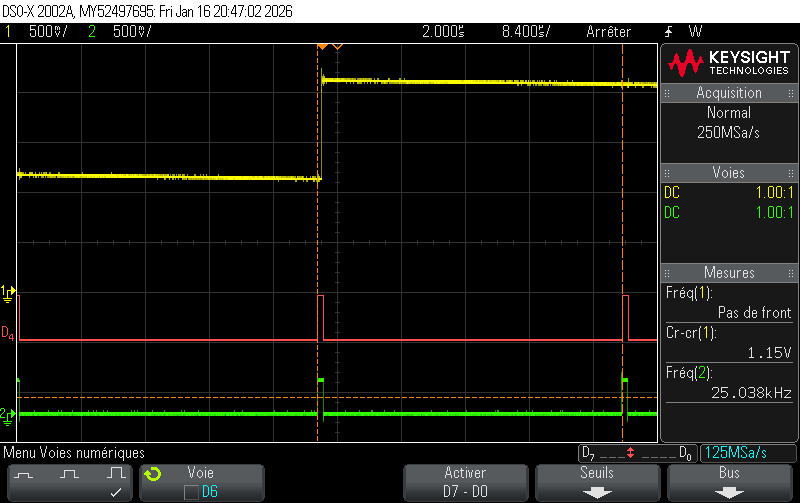
\includegraphics[width=0.65\textwidth]{scope_f8.jpg}
    \caption{Visualisation de l'impulsion IT sur \texttt{VisuPin1}. La largeur de l'impulsion représente le temps réel passé dans la machine à états par rapport à la période $T_{ech}$.}
\end{figure}

\newpage

\section{Fonction 2 : Configuration Dynamique ($F_{ech}$)}

\textbf{La logique :} Permettre à l'utilisateur de saisir une fréquence (ex: $44100\ Hz$) directement dans le menu. Le système doit alors recalculer les registres matériels sans interrompre le programme.

\textbf{Difficulté technique :} Pour maximiser la précision, nous avons choisi de bloquer le Prescaler ($PSC$) à zéro. Cela permet d'utiliser toute la plage du registre $ARR$ ($16$ bits) et ainsi de minimiser l'erreur relative lors de la division de l'horloge système ($80\ MHz$).

\textbf{Code implémenté :}
\begin{lstlisting}
void setFech(uint32_t fech) {
    uint32_t freq_h = 80000000;
    // PSC bloque a zero pour une resolution maximale de ARR
    htim7.Init.Period = (freq_h / (fech)) - 1; 
    if (HAL_TIM_Base_Init(&htim7) != HAL_OK) {
        Error_Handler();
    }
}
\end{lstlisting}

\textbf{Tests et Résultats :}
Nous validons la fréquence demandée en mesurant la période sur la broche de visualisation. Pour $44,1\ kHz$ demandés, nous mesurons bien une période de $22,67\ \mu s$.
\begin{figure}[H]
    \centering
    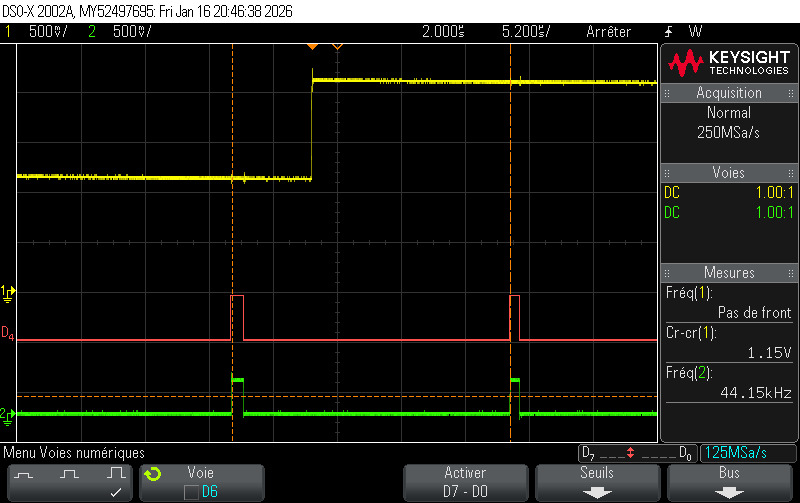
\includegraphics[width=0.65\textwidth]{scope_f7.jpg}
    \caption{Validation de $F_{ech} = 44,1\ kHz$ ($T_{ech} \approx 22,6\ \mu s$). La stabilite est garantie par le mode IT.}
\end{figure}

\newpage

\section{Fonction 3 : Gestion de 2 Zones Mémoires (RAM interne)}

\textbf{Difficulté matérielle (Le $RAM\ Overflow$) :} 
Initialement, nous avons tenté d'allouer deux tableaux de $50\,000$ échantillons \texttt{uint16_t}. Cependant, le STM32L476RG possède seulement $96\ Ko$ de RAM. Le calcul ($50\,000 \times 2\ octets \times 2\ zones = 200\,000\ octets$) a montré que nous dépassions de loin la capacité physique. Le compilateur a renvoyé l'erreur : \texttt{region RAM overflowed}. Nous avons donc réduit l'allocation à \textbf{$20\,000$} par zone ($80\ Ko$ total) pour laisser de la place au système.

\textbf{La logique :} Segmenter la SRAM interne en Zone A et Zone B. Un commutateur logiciel permet de choisir où l'on enregistre et d'où l'on restitue, doublant ainsi l'usage utilitaire de la mémoire vive.

\begin{lstlisting}[caption={Logique de basculement dans enregistreur.c}]
void selectionnerZoneMemoire(donnees_t *pdonnees) {
    if (pdonnees->zoneActive == ZONE_A) {
        pdonnees->zoneActive = ZONE_B;
        printf("\x1B[1;32mZone B active\x1B[0m\r\n");
    } else {
        pdonnees->zoneActive = ZONE_A;
        printf("\x1B[1;32mZone A active\x1B[0m\r\n");
    }
}
\end{lstlisting}

\textbf{Tests et Résultats :}
Nous validons le remplissage indépendant par la console. L'index final de chaque zone est conservé séparément.
\begin{figure}[H]
    \centering
    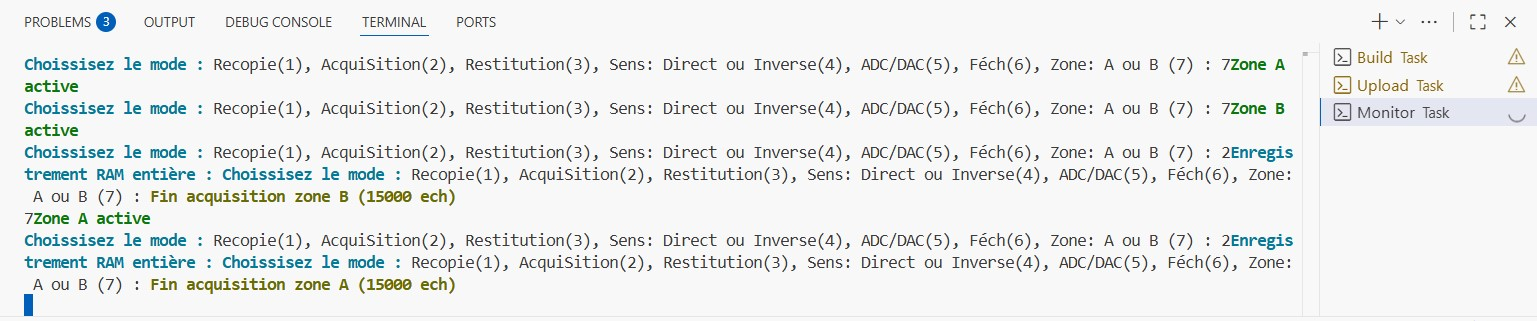
\includegraphics[width=0.85\textwidth]{ZONES.jpg}
    \caption{Preuve console du basculement et du remplissage effectif des deux zones distinctes (limite à $15\,000$ ech ici).}
\end{figure}

\newpage

\section{Fonction 4 : Relecture en Sens Inverse }

\textbf{La logique :} Inverser le signal audio en parcourant le tableau de la fin vers le début. 
Dans la machine à états de restitution, si le sens est \texttt{INVERSE}, l'index démarre à \texttt{indexFinal - 1} et décrémente jusqu'à $0$.

\textbf{Code implémenté (Extrait de modeRestitution) :}
\begin{lstlisting}
if (pdonnees->sensLecture == DIRECT) {
    index++;
    if (index >= indexFinalZone) { index = 0; pdonnees->nbLecture--; }
} else { // Mode INVERSE
    if (index == 0) { index = indexFinalZone - 1; pdonnees->nbLecture--; }
    else { index--; }
}
\end{lstlisting}

\textbf{Tests et Résultats :}
Pour prouver l'inversion sans ambiguïté, nous avons enregistré une \textbf{rampe croissante} (dent de scie).
\begin{itemize}
    \item En mode \texttt{DIRECT}, on observe une pente positive ($0 \to 4095$).
    \item En mode \texttt{INVERSE}, le signal devient une pente négative ($4095 \to 0$), validant mathématiquement l'inversion des index.
\end{itemize}

\begin{figure}[H]
    \centering
    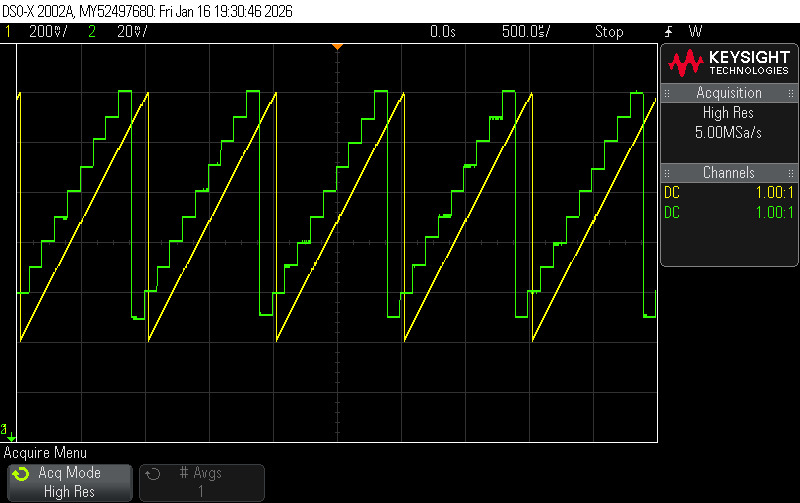
\includegraphics[width=0.45\textwidth]{direct.jpg}
    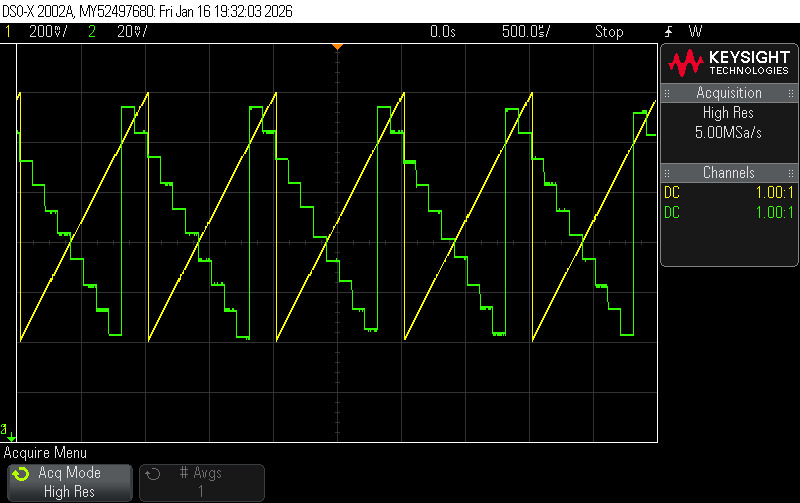
\includegraphics[width=0.45\textwidth]{inverse.jpg}
    \caption{Validation du sens de lecture. À gauche : rampe directe. À droite : rampe inversée (effet reverse).}
\end{figure}

\section{Gestion du Menu et du Bouton Poussoir (Background)}

Le menu intègre désormais les options \textbf{6} ($F_{ech}$) et \textbf{7} (Zone). Le Bouton Poussoir est géré dans le \texttt{while(1)} pour ne pas surcharger l'IT.

\begin{lstlisting}[caption={Menu console avec nouvelles options}]
case '6': 
    printf("Choisissez la frequence d'echantillonnage : ");
    if (fgets(tabfech, 6, stdin) != NULL) { setFech(atoi(tabfech)); }
    break;
case '7': 
    selectionnerZoneMemoire(pdonnees); 
    break;
\end{lstlisting}

\section{Conclusion Générale }


\subsection{Synthèse de l'Architecture}
L'implémentation réussie de la gestion par \textbf{interruptions} via le Timer 7 constitue une vraie amélioration de ce projet. Cette approche a permis de garantir un traitement adapté tout en libérant la CPU.

L'analyse approfondie du fichier \texttt{stm32l4xx_it.c} et du fonctionnement de la couche HAL nous a permis de comprendre que la gestion du drapeau \texttt{UIF} (Update Interrupt Flag) est automatisée par le matériel. Cette compréhension a permis d'épurer le code de la boucle \texttt{while(1)}.

\subsection{Contraintes de tailles}
Face aux limites physiques de la RAM interne ($96$ Ko), nous avons fait preuve d'adaptabilité. Le choix de deux zones de $20000$ échantillons, gérées par une machine à états et des pointeurs spécifiques, a permis de doubler la capacité d'enregistrement sans provoquer de \texttt{RAM overflow}. 

De même, l'optimisation de la fonction \texttt{setFech}, en bloquant le Prescaler (\texttt{PSC}) à zéro, a amélioré l'approche, validée par une erreur relative de fréquence inférieure à $0,1$\% à l'oscilloscope. Toutefois, la fréquence minimale générable est de 1200Hz.

\end{document}